%-------------------------------------------------------------------------------
% APPENDICES 
%-------------------------------------------------------------------------------

\begin{appendices}

\section{Implementation of Boundary Conditions in Julia}

\begin{jllisting}[caption={Boundary reconstruction function by filling in the outer
  two rows and columns of matrix $\Psi$, below the inplace and out of place versions
of this function \vspace{4pt}}]
function constructBC!(Ψ, p::CavityStruct)
    @unpack n, D1, m11, m12, m21, m22, bcleft, bcright, bctop, bcbottom = p.params
    @unpack h1, h2, k1, k2 = p.cache

    @inbounds @views Ψa = Ψ[3:(n - 1), 3:(n - 1)]
    @inbounds @views Ψb = Ψ[3:(n - 1), 2:n]'
    @inbounds @views Dcs = D1[1, 3:(n - 1)]
    @inbounds @views Dce = D1[n + 1, 3:(n - 1)]

    mul!(h1, Ψa, Dcs)
    mul!(h2, Ψa, Dce)

    @inbounds @views @. Ψ[3:(n - 1), 2] = m11 * (bctop[3:(n - 1)] - h1) +
                                          m12 * (bcbottom[3:(n - 1)] - h2)
    @inbounds @views @. Ψ[3:(n - 1), n] = m21 * (bctop[3:(n - 1)] - h1) +
                                          m22 * (bcbottom[3:(n - 1)] - h2)

    mul!(k1, Ψb, Dcs)
    mul!(k2, Ψb, Dce)

    @inbounds @views @. Ψ[2, 2:n] = m11 * (bcleft[2:n] - k1) + m12 * (bcright[2:n] - k2)
    @inbounds @views @. Ψ[n, 2:n] = m21 * (bcleft[2:n] - k1) + m22 * (bcright[2:n] - k2)

    return nothing
end

function constructBC(u, p::CavityStruct)
    @unpack n = p.params

    Ψ = zeros(n + 1, n + 1)
    @inbounds @views Ψ[3:(n - 1), 3:(n - 1)][:] .= u

    constructBC!(Ψ, p)

    return Ψ
end
\end{jllisting}

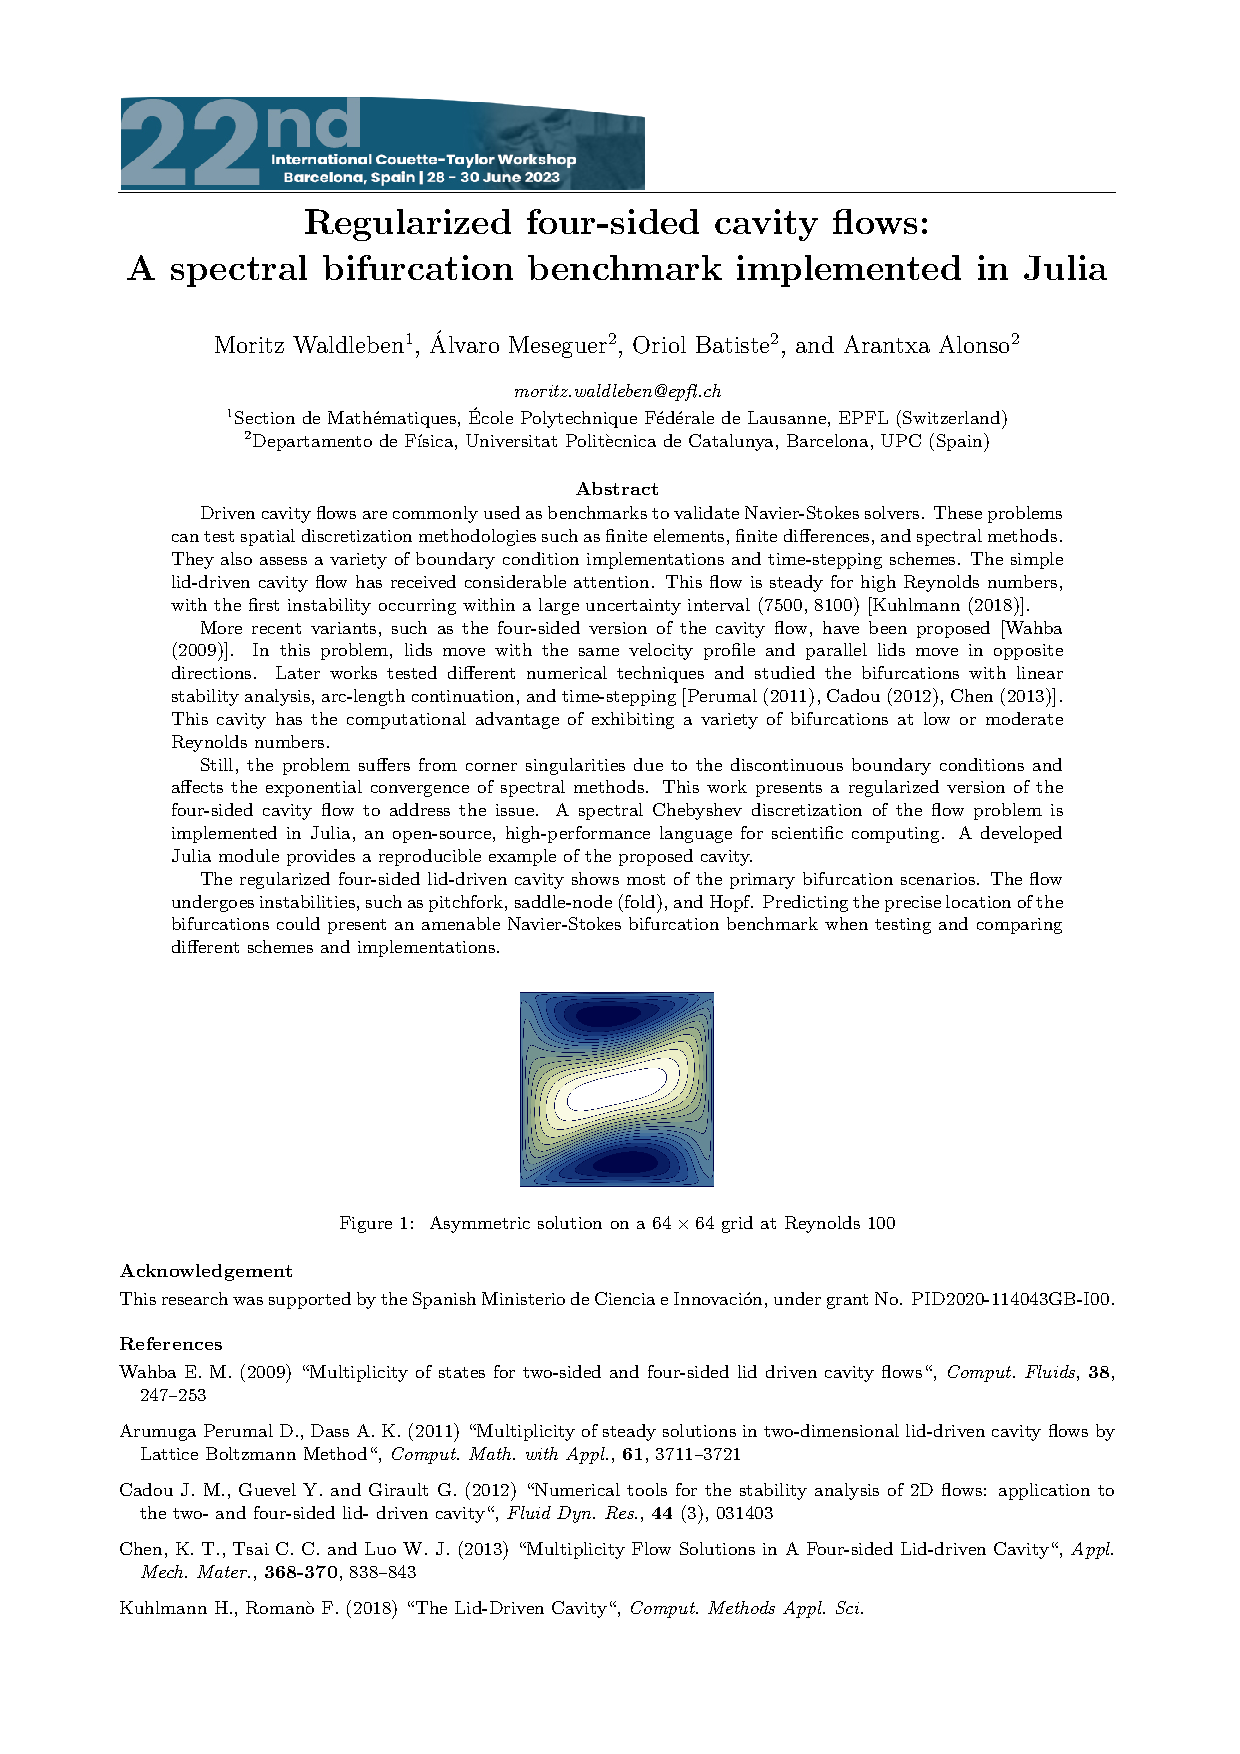
\includepdf[
  scale=0.8,
  offset=75 -75,
  pagecommand=\section{Abstract Conference Presentation at ICTW 2023}
  ]{figs/ictw23_abstract.pdf}

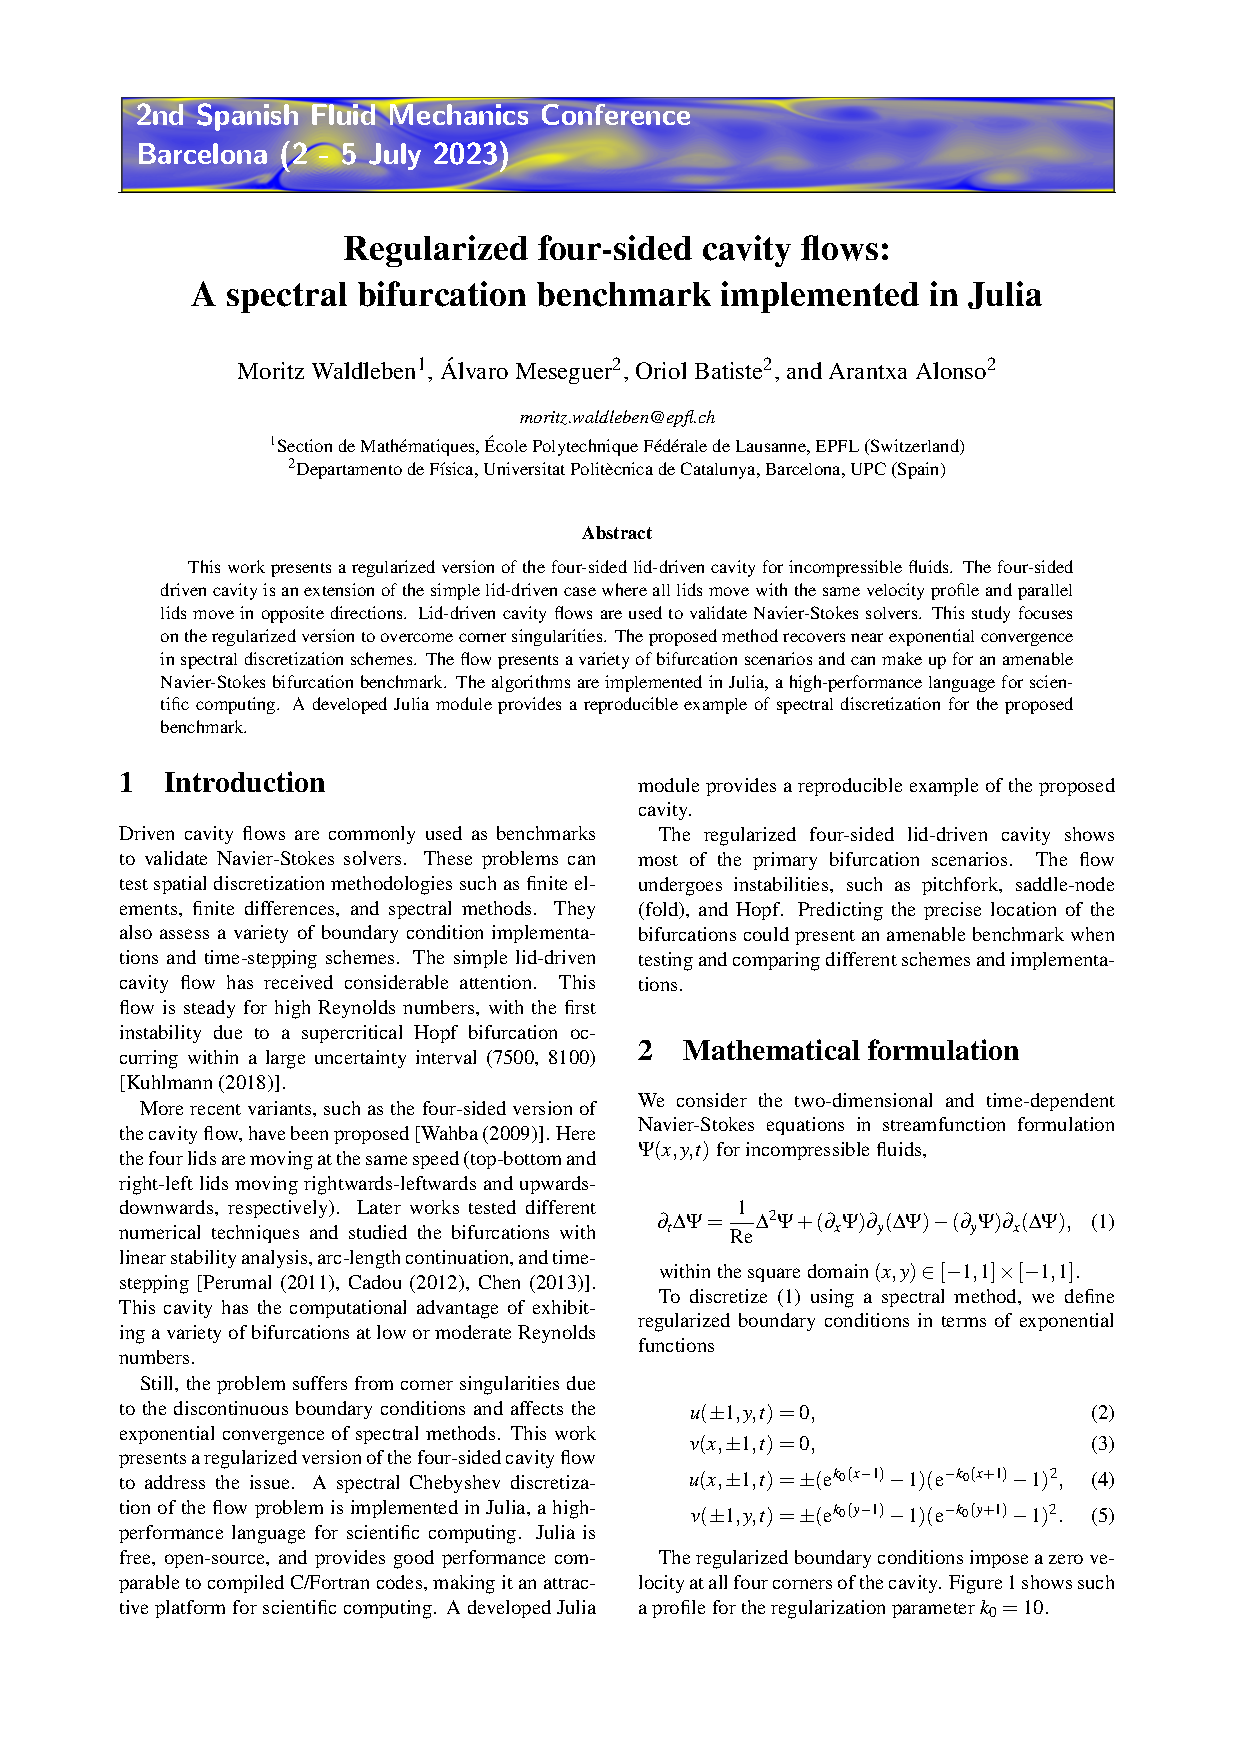
\includepdf[
  scale=0.8,
  pages=1,
  offset=75 -75,
  pagecommand=\section{Abstract Conference Presentation at SFMC 2023}
]{figs/sfmc23_abstract.pdf}
\includepdf[
  scale=0.8,
  pages=2,
  offset=75 -75,
  pagecommand={},
  trim=0 2cm 0 2cm,
  clip
]{figs/sfmc23_abstract.pdf}

\end{appendices}
